\documentclass[11pt]{article}
\usepackage[margin=1in]{geometry}
\usepackage{amsmath,amssymb}
\usepackage{graphicx}
\usepackage{booktabs}
\usepackage{longtable}
\usepackage{xcolor}
\usepackage{tikz}
\usetikzlibrary{arrows.meta,positioning,shapes.geometric,fit,calc}
\usepackage{hyperref}
\usepackage{caption}
\usepackage{subcaption}

\setlength{\emergencystretch}{3em}
\newcommand{\Scap}{S_{\mathrm{cap}}}
\newcommand{\Smin}{S_{\mathrm{in}}}
\newcommand{\Qsafe}{Q_{\mathrm{safe}}}
\newcommand{\code}[1]{\texttt{#1}}
\newcommand{\terclo}{640}
\newcommand{\tercHi}{1149}
\newcommand{\demandvol}{644}
\newcommand{\meanrunoff}{1093}


\title{Functional Environmental Flows from Reinforcement Learning:\\
       a Proof of Concept on a Lake McClure--like Reservoir\\
       with OpenHydroQual as the Simulator}
\author{OpenHydroQual-RL working notes}
\date{\today}

\begin{document}
\maketitle

\begin{abstract}
Environmental flow (e-flow) requirements below dams are usually
\emph{prescriptive}: a fixed release schedule, chosen in advance for each
water-year type. This note tests the alternative proposed in the
``DRL for e-flows'' outline: put the ecological objectives into the
\emph{reward} of a reinforcement-learning (RL) agent and let the agent
decide, day by day, how to release water. We build a reservoir patterned
on Lake McClure on the Merced River (California), drive it with the
observed daily unimpaired inflow for water years 1989--2025, and simulate
it with OpenHydroQual (OHQ) through its Python bindings. Each day the agent
chooses the river release and the irrigation delivery. The ecological
objective follows the five functional-flow components of the California
Environmental Flows Framework (fall pulse, wet-season baseflow, peak
flows, spring pulse and recession, dry-season baseflow). The targets are
derived from the river's own unimpaired hydrology, separately for dry,
moderate and wet years. We compare four operating modes on the 2017--2025
test period, which spans a record wet year, a drought and another wet year:
(1) a regulatory minimum instream flow, (2) a prescribed functional-flow
hydrograph, (3) functional flows in the reward, and (4) functional flows
plus hydropower in the reward. Results are reported as irrigation
reliability, flood days, energy and a functional-flow score between 0 and
1.
\end{abstract}

\tableofcontents
\newpage

%=====================================================================
\section{Motivation and what this note does}
\label{sec:intro}

Most e-flow requirements are \emph{static}. A schedule of minimum flows,
sometimes with pulses, is fixed in a licence and indexed to the water-year
type. Static rules are easy to write down and to enforce, but they ignore
information that operators actually have: the state of the reservoir, the
snowpack forecast, and whether a natural storm is passing anyway. Under
climate change the hydrology that a static schedule was designed for also
drifts away from the hydrology it has to work with.

An \emph{adaptive} rule maps what the operator knows today to a release
today. Reinforcement learning is a general way to find such a rule by
trial and error in a simulator. We specify \emph{what} we want (the reward)
and the algorithm searches for \emph{how} to operate. The question the
outline poses is whether e-flows can be expressed as part of that reward,
so that an e-flow-friendly operation emerges from the optimization instead
of being prescribed. The outline's Scenario~3, ``reward-function
functional flows'', is its core novelty.

This note is a working proof of concept of that idea. It follows the
outline's four scenarios on a single reservoir:

\begin{enumerate}
\item \textbf{Minimum instream flow} (MIF). A regulatory floor on the river
  flow; the agent (or rule) manages supply and floods above it.
\item \textbf{Prescribed functional flows.} A fixed functional-flow
  hydrograph for each year type replaces the MIF floor.
\item \textbf{Functional flows in the reward.} No floor. Every functional-flow
  component is scored daily and added to the reward.
\item \textbf{Multi-objective.} Scenario 3 plus hydropower in the reward
  (flood control is in every scenario).
\end{enumerate}

\noindent The general RL background (states, actions, rewards, value
functions, the PPO algorithm) is explained step by step in the companion
tutorial report \emph{Learning Reservoir Operating Rules with Reinforcement
Learning} (\code{report/main.pdf}). Here we only summarize what is needed
(Section~\ref{sec:rl}) and concentrate on the e-flow problem.

%=====================================================================
\section{The system}
\label{sec:system}

\subsection{A Lake McClure--like reservoir}
Lake McClure (New Exchequer Dam) on the Merced River stores about
1.02~million acre-feet (1264~hm$^3$). It is operated by the Merced
Irrigation District for irrigation, hydropower and flood control, under
FERC and other in-stream flow requirements. We do \emph{not} attempt a
faithful model of the real system (no McSwain/Merced Falls re-regulation,
no evaporation, simplified head and flood rules). The aim is a stylized
system with realistic hydrology, demand and scale, so that the trade-offs
are real ones. Figure~\ref{fig:schematic} shows the model.

\begin{figure}[h]
\centering
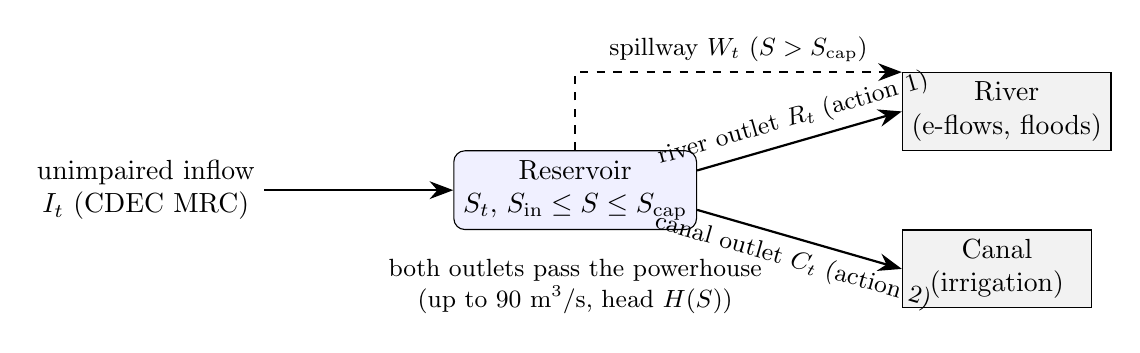
\begin{tikzpicture}[node distance=1.2cm and 2.2cm,
  box/.style={draw, rounded corners, minimum width=2.6cm, minimum height=1cm, align=center, fill=blue!6},
  sink/.style={draw, minimum width=2.4cm, minimum height=0.8cm, align=center, fill=gray!10},
  arr/.style={-{Stealth[length=3mm]}, thick}]
\node[box] (res) {Reservoir\\ $S_t$, $\Smin\le S\le\Scap$};
\node[left=2.4cm of res, align=center] (in) {unimpaired inflow\\ $I_t$ (CDEC MRC)};
\node[sink, right=2.6cm of res, yshift=1.0cm] (river) {River\\(e-flows, floods)};
\node[sink, right=2.6cm of res, yshift=-1.0cm] (canal) {Canal\\(irrigation)};
\draw[arr] (in) -- (res);
\draw[arr] (res.east) ++(0,0.25) -- node[above, sloped, font=\small] {river outlet $R_t$ (action 1)} (river.west);
\draw[arr] (res.east) ++(0,-0.25) -- node[below, sloped, font=\small] {canal outlet $C_t$ (action 2)} (canal.west);
\draw[arr, dashed] (res.north) |- node[above, pos=0.75, font=\small] {spillway $W_t$ ($S>\Scap$)} (river.north west);
\node[below=0.25cm of res, font=\small, align=center] {both outlets pass the powerhouse\\(up to 90 m$^3$/s, head $H(S)$)};
\end{tikzpicture}
\caption{The model. Every day the agent sets the river release $R_t$ and
the canal delivery $C_t$. The spillway is uncontrolled. In OHQ the
reservoir is a \code{Reservoir} block, the three receivers are
\code{fixed\_head} blocks whose storage accumulates the delivered volume,
and the outlets are \code{Reservoir\_link\_rule} links.}
\label{fig:schematic}
\end{figure}

\subsection{Data}
All data are public daily series (Table~\ref{tab:data}), fetched by
\code{prepare\_merced.py}.

\begin{table}[h]
\centering\small
\begin{tabular}{@{}llll@{}}
\toprule
Series & Source & Use & Period \\
\midrule
Full natural (unimpaired) flow, Merced R.\ nr Merced Falls & CDEC MRC, sensor 8 & inflow $I_t$, targets & WY1989--2025\\
Lake McClure storage & CDEC EXC, sensor 15 & initial storage of test windows & 1988--2025\\
Lake McClure outflow & CDEC EXC, sensor 23 & irrigation demand & 1994--2025\\
Merced R.\ near Snelling (below the diversions) & USGS 11272500 & demand; historical river flow & WY1989--2010\\
\bottomrule
\end{tabular}
\caption{Data. The irrigation demand is the observed diversion, i.e.\
reservoir outflow minus the river flow below the Crocker--Huffman
diversion dam (WY1994--2010).}
\label{tab:data}
\end{table}

\noindent Water years (WY) run October~1 to September~30. Leap days are
dropped, so every year has 365 daily steps, with day $d=0$ on October~1.
The mean unimpaired runoff of the training years (WY1989--2016) is
\meanrunoff~hm$^3$/yr and the irrigation demand is \demandvol~hm$^3$/yr,
so in an average year a little over half of the inflow is wanted for
irrigation, and in a dry year all of it and more (Figure~\ref{fig:volumes}).

\begin{figure}[h]
\centering
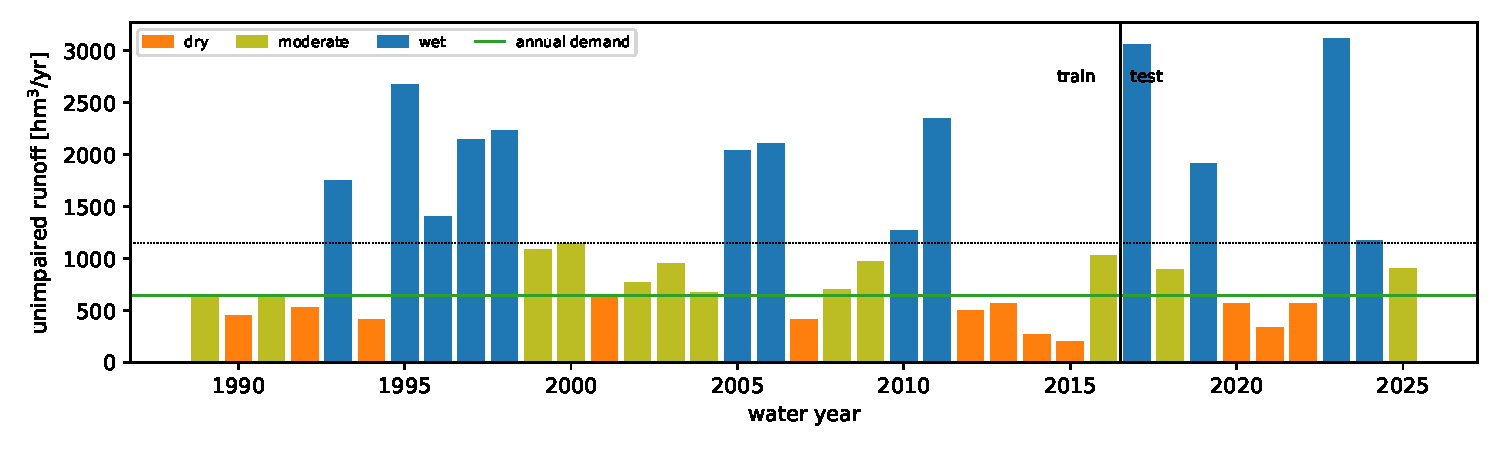
\includegraphics[width=\textwidth]{figures/annual_volumes.pdf}
\caption{Annual unimpaired runoff and year types. The dotted lines are the
terciles of the training years (\terclo{} and \tercHi{}~hm$^3$), which
define dry, moderate and wet years. The green line is the annual
irrigation demand. The test period WY2017--2025 contains the wettest year
of the record (2023), the 2020--2022 drought and the wet 2017.}
\label{fig:volumes}
\end{figure}

\subsection{Parameters, demand, flood control and minimum flow}

\begin{table}[h]
\centering\small
\begin{tabular}{@{}llp{7.5cm}@{}}
\toprule
Symbol & Value & Meaning\\
\midrule
$\Scap$ & 1264 hm$^3$ & capacity (1.02 MAF); spillway opens above it\\
$\Smin$ & 80 hm$^3$ & inactive pool; both outlets taper to zero just above it (the observed minimum was 78~hm$^3$ in 2015)\\
$R_{\max}$ & 300 m$^3$/s & river outlet capacity\\
$\Qsafe$ & 170 m$^3$/s & safe channel capacity (6000 cfs)\\
$D_d$ & Fig.~\ref{fig:demand} & irrigation demand on water-year day $d$; peak $D_{\max}=50$ m$^3$/s\\
$S_{\mathrm{toc}}(d)$ & Fig.~\ref{fig:demand} & flood-control rule curve: 432~hm$^3$ (350~kAF) of flood space Nov~1--Mar~1\\
$H(S)$ & 70--140 m & gross head, $70+70\,x^{0.6}$ with $x=(S-\Smin)/(\Scap-\Smin)$\\
$P$ & $\le$ 94.5 MW & $P=\rho g\,\eta\,\min(R+C,\,90)\,H$, $\eta=0.88$\\
\bottomrule
\end{tabular}
\caption{System parameters.}
\label{tab:params}
\end{table}

\begin{figure}[h]
\centering
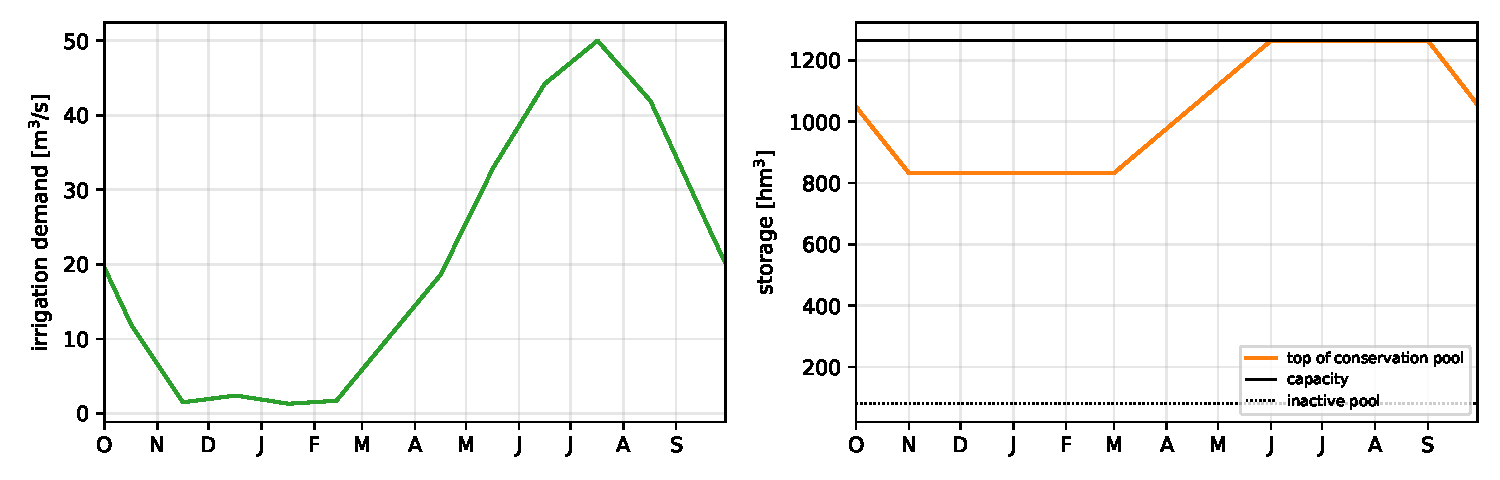
\includegraphics[width=0.95\textwidth]{figures/demand_rulecurve.pdf}
\caption{Left: daily irrigation demand (mean observed diversion per month,
interpolated). Right: flood-control rule curve used by the rule-based
baselines and given to the agent as an observation.}
\label{fig:demand}
\end{figure}

\noindent The \textbf{minimum instream flow} of Scenario~1 is stylized after
the FERC licence and the Davis--Grunsky requirements on the Merced: 75~cfs
in late October, 180~cfs from November to March, 75~cfs in April and May,
and 25~cfs from June to mid-October, with 60\% of these in dry years.
Figure~\ref{fig:targets} shows it in blue.

%=====================================================================
\section{Functional flows as numbers}
\label{sec:ff}

\subsection{The five components}
The California Environmental Flows Framework (CEFF; Yarnell et al.\ 2020)
describes a healthy hydrograph of a California river by five
\emph{functional-flow components}, each tied to ecological functions:
\begin{description}
\item[Fall pulse (FA).] The first rains of autumn. It flushes fine sediment and
  cues salmon migration and spawning.
\item[Wet-season baseflow (WB).] Sustained winter flow. It keeps habitat wetted
  for rearing.
\item[Peak flows (PK).] Large, infrequent floods. They move the bed, scour
  vegetation and connect the floodplain.
\item[Spring pulse and recession (SP).] The snowmelt pulse and its gradual
  decline. Spawning and seed dispersal follow it, and fish are stranded if it
  stops abruptly.
\item[Dry-season baseflow (DS).] Low summer flow. It sets the summer habitat
  and water temperature.
\end{description}

\noindent For an RL agent, ``a healthy hydrograph'' must become a number it
can earn every day. We give each component a calendar window, a target, and
a score. CEFF detects the timing of each component from the hydrograph; we
use fixed windows to keep the rules readable (Table~\ref{tab:windows}).

\begin{table}[h]
\centering\small
\begin{tabular}{@{}llll@{}}
\toprule
Component & Window & Requirement & Year score $\in[0,1]$\\
\midrule
FA & Oct 15 -- Dec 15 & $\ge D_{FA}$ days with $Q\ge Q_{FA}$ & $\min(1,\ \sum_d c_d/D_{FA})$\\
WB & Dec 16 -- Mar 31 & $Q\ge Q_{WB}$ every day & mean of $c_d$\\
PK & Dec 1 -- Apr 30 & $\ge D_{PK}$ days with $Q\ge Q_{PK}$ & $\min(1,\ \sum_d c_d/D_{PK})$\\
SP & Apr 1 -- May 31 & $\ge D_{SP}$ days with $Q\ge Q_{SP}$ & $\tfrac12\min(1,\sum_d c_d/D_{SP})$\\
   & Apr 15 -- Jun 30 & decline of the 7-day mean flow $\rho_d\le r_{\max}$ & $+\tfrac12$ mean recession credit\\
DS & Jul 1 -- Oct 14 & $Q\ge Q_{DS}$ every day & mean of $c_d$\\
\bottomrule
\end{tabular}
\caption{Functional-flow components as used here ($Q$ is the river flow below
the reservoir, including spill). Day credit
$c_d=\mathrm{clip}\big((Q_d/Q_k-0.9)/0.09,\,0,\,1\big)$: full at 99\% of the
target or more, falling linearly to zero at 90\%. Recession credit is 1 for
$\rho_d\le r_{\max}$ and falls linearly to 0 at $\rho_d=2r_{\max}$.}
\label{tab:windows}
\end{table}

\noindent Two choices make the score robust to small release errors.
Graded credit means a release 2\% short of a target loses a little, not a
whole day. Measuring the recession on the trailing 7-day mean flow,
$\rho_d=(\bar Q_{d-1}-\bar Q_d)/\bar Q_{d-1}$, matches how $r_{\max}$ is
derived from the natural flow (below). A first version with pass/fail
days and raw daily declines turned out to be so sensitive that day-to-day
release jitter of a few percent failed most of the spring
(Section~\ref{sec:training}).

\noindent The \textbf{functional-flow (FF) score} of a year is the mean of
the component scores that apply. A pulse with a required duration of zero
(peak flows in dry years) does not apply. A score of 1 means every
component is fully met.

\subsection{Targets from the river's own natural flow}
Following CEFF, targets come from the unimpaired hydrology of the same river
over the training years, for each year type:
\begin{itemize}
\item $Q_{WB}$: median over the years of the window's 10th-percentile flow (CEFF
  \code{Wet\_BFL\_Mag\_10});
\item $Q_{DS}$: 25th percentile over the years of the window's median flow (the
  lower end of the natural range of \code{DS\_Mag\_50});
\item $Q_{FA}$: 25th percentile of the natural fall maxima, $D_{FA}=2$~days;
\item $Q_{SP}$: half the median natural spring maximum; $D_{SP}$ the median number
  of natural days above it, capped at 7;
\item $Q_{PK}$: the median annual peak (about the 2-year flood) capped at
  $0.8\,\Qsafe$, because a regulated river cannot be asked to flood its own
  channel; $D_{PK}$ is the median number of natural days above it (capped at 7);
\item $r_{\max}$: 90th percentile of the natural daily declines of the 7-day mean
  flow during the recession window (about 10\%/day, close to the CEFF
  guidance for Sierra snowmelt rivers).
\end{itemize}
Table~\ref{tab:targets} gives the values and Figure~\ref{fig:targets} shows
them against the natural hydrographs. The unimpaired flow itself scores
only 0.76--0.83, because natural years scatter around the targets: a
natural dry year often has no fall pulse. A regulated river that
scores near 0.8 is therefore about as ``functional'' as the natural one
\emph{by these metrics}.

\begin{table}[h]
\centering\small
\begin{tabular}{@{}llrrr@{}}
\toprule
Target & Unit & dry & moderate & wet\\
\midrule
Fall pulse magnitude $Q_{FA}$ & m$^3$/s & 10.96 & 10.24 & 31.38 \\
Fall pulse duration $D_{FA}$ & d & 2 & 2 & 2 \\
Wet-season baseflow $Q_{WB}$ & m$^3$/s & 2.80 & 7.54 & 10.77 \\
Peak flow magnitude $Q_{PK}$ & m$^3$/s & 136.00 & 136.00 & 136.00 \\
Peak flow duration $D_{PK}$ & d & 0 & 1 & 7 \\
Spring pulse magnitude $Q_{SP}$ & m$^3$/s & 44.64 & 75.23 & 120.25 \\
Spring pulse duration $D_{SP}$ & d & 7 & 7 & 7 \\
Max.\ recession rate $r_{\max}$ & 1/d & 0.10 & 0.10 & 0.10 \\
Dry-season baseflow $Q_{DS}$ & m$^3$/s & 0.34 & 1.67 & 4.11 \\
\midrule
Prescribed hydrograph volume & hm$^3$/yr & 109 & 240 & 454 \\
Minimum instream flow volume & hm$^3$/yr & 53 & 89 & 89 \\
FF score of the unimpaired flow & -- & 0.76 & 0.78 & 0.83 \\

\bottomrule
\end{tabular}
\caption{Functional-flow targets by year type (from WY1989--2016 unimpaired
flow), volume of the prescribed hydrograph and of the minimum instream
flow, and the score that the unimpaired flow itself gets.}
\label{tab:targets}
\end{table}

\begin{figure}[h]
\centering
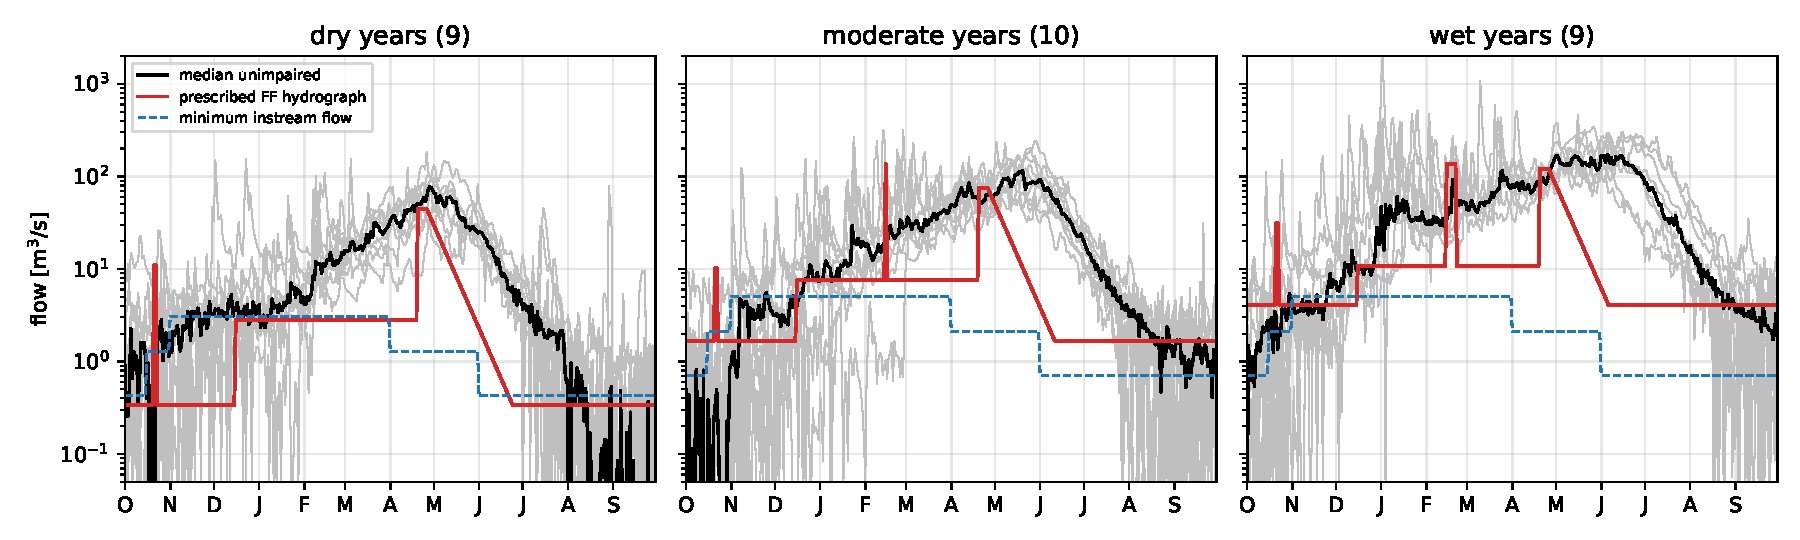
\includegraphics[width=\textwidth]{figures/natural_targets.pdf}
\caption{Unimpaired daily flow of the training years (gray; median in black),
the prescribed functional-flow hydrograph used in Scenario~2 (red), and the
minimum instream flow of Scenario~1 (blue, dashed). Log scale.}
\label{fig:targets}
\end{figure}

\subsection{The prescribed hydrograph (Scenario 2)}
The prescriptive alternative turns the targets into a fixed release
schedule for each year type, met by construction:
baseflow floors in their windows, a fall pulse on October~21, a peak-flow
block on February~15 (moderate and wet years), and a spring pulse on
April~20 followed by a recession at $0.8\,r_{\max}$ down to the
dry-season floor (red lines in Figure~\ref{fig:targets}). It costs
109/240/454~hm$^3$ of river water in dry/moderate/wet years, against
53--89~hm$^3$ for the minimum instream flow.

\subsection{Year type under uncertainty}
\label{sec:yeartype}
Targets depend on the year type, but the type of the current year is not
known until it is over. As in California practice, the operator works with
a \emph{declared} type based on the runoff forecast. We imitate a
Bulletin-120 forecast: the remaining runoff of the water year is
known with a log-normal error. The error's spread falls from 50\% before
February to 15\% in April and 5\% in June, and the error is redrawn every
month. On each day the declared type is the tercile class of
(runoff so far $+$ forecast of the rest). Daily targets follow that day's
declaration, and the year's score uses the May~1 declaration. A prescribed
schedule therefore sometimes releases a ``dry'' winter baseflow in what turns
out to be a moderate year, which is the real cost of deciding early.

%=====================================================================
\section{The reinforcement-learning problem}
\label{sec:rl}

\subsection{In one paragraph}
An RL \emph{agent} (a small neural network, the \emph{policy}) looks at the
\emph{state} of the system each day and chooses an \emph{action}. The
simulator advances one day and returns a \emph{reward}. Training adjusts the
network so that the expected sum of discounted rewards,
$\mathbb{E}\big[\sum_t \gamma^t r_t\big]$, is as large as possible.
Nothing about how to operate is programmed in. Everything the agent learns
comes from the reward and the simulated consequences of its own choices.
The companion report explains this in detail.

\subsection{What the agent sees (state)}
The observation $o_t$ has 18 entries, all scaled to order one:
storage $S_t/\Scap$; today's inflow and its 7- and 30-day means (as
$\log(1+I/10)$); the season ($\sin$, $\cos$ of $2\pi d/365$); the forecast
of the remaining water-year runoff$/\Scap$; yesterday's river flow; today's
demand$/D_{\max}$; today's \emph{reference} river flow (in action units:
the hard floor in Scenarios 1--2, the prescribed functional-flow schedule of
the declared year type in Scenarios 3--4, where it is only a hint the agent
may ignore); the declared
year type (three 0/1 flags); the progress of the fall, peak and spring
pulses this year (days achieved$/$days required); the flood space
$(S_{\mathrm{toc}}-S_t)/\Scap$; and a spill-risk indicator
$(S_t+\text{forecast}-\Scap)/\Scap$. The pulse-progress entries are needed
because the pulse rewards depend on what has already been achieved this
year. Without them the reward would not be a function of the observed
state.

\subsection{What the agent decides (actions)}
Two numbers $a_1,a_2\in[-1,1]$:
\begin{align}
R_t &= R_{\min}\left(\frac{R_{\max}}{R_{\min}}\right)^{(a_1+1)/2} , &
C_t &= D_d\,\min\!\big(1,\ 0.6\,(a_2+1)\big),
\end{align}
with $R_{\min}=0.1$ and $R_{\max}=300$~m$^3$/s. The river release is on a
log scale because the targets range from 0.3~m$^3$/s (dry-season baseflow)
to 136~m$^3$/s (peak flow): an error in $a_1$ is then the same
\emph{relative} flow error at every level. An earlier version with
$R_t\propto(a_1+1)^2$ could not hold small baseflows accurately enough. Delivery is a fraction of today's
demand, reaching 100\% at $a_2\ge 2/3$. In Scenarios 1 and 2 the river
release is raised to the floor if needed, $R_t\leftarrow\max(R_t, F_t)$.
Both outlets taper to zero just above the inactive pool, so the reservoir
cannot be overdrawn.

\subsection{What the agent is rewarded for}
\label{sec:reward}
With $Q_t=R_t+W_t$ the river flow (release plus spill), the daily reward is
the sum of these terms:
\begin{align}
r^{\mathrm{sup}}_t &= -w_s\left(\frac{(D_d-C_t)^+}{D_{\max}}\right)^2
  &&\text{irrigation shortage (squared: many small cuts beat one big one)}\\
r^{\mathrm{fl}}_t &= -w_f\,\frac{(Q_t-\Qsafe)^+}{\Qsafe}
  &&\text{flooding below the dam}\\
r^{\mathrm{ff}}_t &= -w_{\mathit{ff}}\sum_{k\in\{WB,DS\}}\mathbb{1}_k(d)\,\frac{1-c_t^{(k)}}{N_k}
  && \text{baseflow days missed}\nonumber\\
  &\quad+ \sum_{k\in\{FA,PK,SP\}} \omega_k\,w_{\mathit{ff}}\,\mathbb{1}_k(d)\,\Delta\!\min\!\Big(1,\frac{n_k}{D_k}\Big)
  && \text{pulse progress, } n_k\leftarrow n_k+c_t^{(k)}\nonumber\\
  &\quad- \tfrac12 w_{\mathit{ff}}\,\mathbb{1}_{REC}(d)\,\frac{1}{N_{REC}}\min\!\left(1,\frac{(\rho_t-r_{\max})^+}{r_{\max}}\right)
  && \text{too-fast recession of the 7-day mean}\\
r^{\mathrm{hp}}_t &= w_h\,P_t/P_{\max} &&\text{energy}
\end{align}
where $\mathbb{1}_k(d)$ is one inside the window of component $k$, $N_k$ is
the number of days in that window, $c_t^{(k)}$ is the day credit of
Table~\ref{tab:windows}, $\omega_{FA}=\omega_{PK}=1$, $\omega_{SP}=\tfrac12$,
and $n_k$ accumulates the day credits of pulse $k$ this year.

\textbf{The functional-flow reward is the score, paid daily.} Summed over a
year, $r^{\mathrm{ff}}$ equals $w_{\mathit{ff}}$ times the sum of the
component scores, minus a constant. Every component is worth
$w_{\mathit{ff}}=5$ per year, and the agent is paid for exactly what it is
later judged on. An earlier version used a squared baseflow shortfall,
$-\big((Q_k-Q_t)^+/Q_k\big)^2$, instead. A 15\% shortfall then cost almost
nothing in reward, but it zeroes the day in the score. PPO duly learned to
shave baseflows to save water: its reward rose above the rule's while its
functional-flow score fell from 0.85 to 0.70. We met the same trap in the
stormwater-pond problem of the companion report. When the reward and the
evaluation measure differ, RL optimizes the reward.

The pulse term pays the \emph{increase} of the progress $\min(1,n_k/D_k)$
and never pays the same progress twice. A pulse therefore earns at most
$\omega_k w_{\mathit{ff}}$ per year, even when the declared year type
(and with it $D_k$) changes during the year. Partial pulses earn partial
credit. Two loopholes in earlier versions are worth recording, because RL
finds such holes quickly. Near-miss days were paid without counting
toward the duration, so hovering just below the target paid more than
completing the pulse. And the payment per day was $w_p/D_k$ with the
\emph{current} $D_k$, so a change of year type mid-pulse paid twice.
Scenarios combine the terms as follows:
\begin{center}\small
\begin{tabular}{@{}lll@{}}
\toprule
Scenario & Hard river floor & Reward\\
\midrule
1 MIF & minimum instream flow & $r^{\mathrm{sup}}+r^{\mathrm{fl}}$\\
2 Prescribed & prescribed FF hydrograph & $r^{\mathrm{sup}}+r^{\mathrm{fl}}$\\
3 FF reward & none & $r^{\mathrm{sup}}+r^{\mathrm{fl}}+r^{\mathrm{ff}}$\\
4 Multi & none & $r^{\mathrm{sup}}+r^{\mathrm{fl}}+r^{\mathrm{ff}}+r^{\mathrm{hp}}$\\
\bottomrule
\end{tabular}
\end{center}
The weights are $w_s=5$, $w_f=1$, $w_{\mathit{ff}}=5$ and $w_h=0.1$.
They are value judgements, not physics. A 15\% shortage spread over the
irrigation season costs about $-16$ per year, and raising the
functional-flow score from 0 to 1 is worth $5\times$(number of components),
i.e.\ 20--25 per year. Changing the weights traces out different points on the
supply--ecology trade-off (Section~\ref{sec:discussion}).

To compare policies that were trained or operated under different
scenarios, we use one common yardstick, $J_{\mathrm{ff}}$: the mean
per-year sum of $r^{\mathrm{sup}}+r^{\mathrm{fl}}+r^{\mathrm{ff}}$, i.e.\
the Scenario~3 reward, computed for every policy.

\subsection{Episodes, discounting and the end of an episode}
An episode is three consecutive water years, starting from a random
training year (WY1989--2016) and a random storage between 30\% and 85\% of
capacity. Three years let carry-over storage matter, as in drought
sequences. The discount factor is $\gamma=0.995$, an effective horizon of
about 200 days. That is long enough to see that water stored in winter
pays off in summer.

The end of an episode is a \emph{time limit}, not the end of the world.
The reservoir would keep operating. Treating the last day as terminal would
teach the agent that water left in storage at the end is worthless, and it
would empty the reservoir. We therefore \emph{bootstrap} at the time limit:
the critic's estimate of the value of the final state is added to the last
reward ($r_T\leftarrow r_T+\gamma\,V(s_{T+1})$). This addition to the
training code (\code{train\_ppo.py}, the \code{boot} entries) is the standard
fix for time limits.

%=====================================================================
\section{The simulator: one OHQ run per day}
\label{sec:ohq}
Every decision step builds and solves a one-day OHQ model through
\code{openhydroqual\_py} (\code{McClureBackend} in \code{ohq\_eflows\_env.py}):
\begin{itemize}
\item a \code{Reservoir} block with the day's storage and a constant inflow time series;
\item three \code{fixed\_head} receivers (River, Canal, Spill), whose storage
  accumulates the delivered volume, so day-mean flows are read exactly;
\item two \code{Reservoir\_link\_rule} outlets with $Q_{\max}$ set to the
  action and a linear taper over the 1\% of capacity above $\Smin$;
\item a third \code{Reservoir\_link\_rule} as spillway, opening from $\Scap$
  to $1.01\,\Scap$ with a capacity of 5000~m$^3$/s;
\item solver step 0.1~d, fixed (\code{max\_timestep\_increase\_factor}=1),
  one solver thread per model (\code{n\_threads}=1), because 24 models run
  in parallel.
\end{itemize}
The daily water balance $S_{t+1}=S_t+(I_t-R_t-C_t-W_t)\,\Delta t$ closes to
about $10^{-4}$~hm$^3$, i.e.\ $10^{-7}$ of the storage. One worker runs
about 150 simulated days per second. With 24 parallel workers training
runs at about 1400 days per second, so four million simulated days
(about 11{,}000 years of operation) take under an hour.

%=====================================================================
\section{How the agent is trained}
\label{sec:training}
We use proximal policy optimization (PPO), the same actor--critic algorithm
as in the companion report. An \emph{actor} network maps $o_t$ to the mean of
a Gaussian over actions, and a \emph{critic} network estimates the value
$V(o_t)$. Training repeats: 24 workers each run the current policy for 512
days; advantages are computed with GAE ($\lambda=0.95$); both networks are
updated for 5 epochs with the clipped PPO objective (learning rate
$5\times10^{-5}$, rewards scaled by the running standard deviation of the
discounted return). Getting PPO to improve on the rule at all took several
attempts. The lessons are as useful as the result:

\begin{enumerate}
\item \textbf{Learn a correction to the rule, not the rule itself
  (residual policy).} Our first attempt cloned the tuned prescriptive rule
  into the actor by regression and then ran PPO. The clone was never exact:
  its action errors of about $\pm6\%$ in flow cost 5.7 of the rule's 7.85
  reward points per year, and PPO only won part of that back. In the final
  set-up the agent's action is a \emph{correction} added to the rule's
  action, $a_t=\mathrm{clip}\big(a^{\mathrm{rule}}(o_t)+\delta_\theta(o_t)\big)$,
  and the actor starts at $\delta_\theta\equiv0$. Training therefore starts
  from the rule exactly. The correction has full authority, $\delta\in[-1,1]$,
  so the agent can override the rule completely wherever that pays. This is
  ``residual RL''. The rule supplies the calendar of a functional-flow
  hydrograph, which is hard to learn from scratch, and RL adapts it to
  storage, forecasts and the passing hydrology.
\item \textbf{Exploration noise must not create penalties by itself.} PPO
  explores by adding Gaussian noise to the action. On a log-scale release,
  noise of standard deviation 0.018 is $\pm7\%$ daily flow jitter. With the
  first, pass/fail version of the functional-flow reward, that jitter alone
  cost 8.6 points per year (the rule's whole reward was 7.6): mostly
  recession violations, because the prescribed recession ran at 95\% of
  the limit. PPO then learned to cope with its own noise, which made the
  noise-free policy \emph{worse}. The graded credit, the 7-day-mean
  recession and a recession at 80\% of the limit cut the noise cost to
  0.85 points per year at standard deviation 0.01, which is the
  exploration level used.
\item \textbf{Keep the best snapshot, judged on the real objective.} A
  checkpoint is saved every 18 updates. Each one is run
  \emph{deterministically} (no exploration noise) on five training-period
  windows (starting 1990, 1996, 2002, 2008, 2012), and the one with the
  highest mean reward per year is kept. The test years are never used for
  any choice.
\end{enumerate}

%=====================================================================
\section{Baselines}
\label{sec:baselines}
Each scenario has a rule-based baseline, a \emph{standard operating policy
with hedging}:
\begin{itemize}
\item river: today's floor (MIF or prescribed hydrograph); in Scenarios 3--4,
  which have no floor, the prescribed hydrograph, so the baseline is the
  prescriptive operation scored with the functional-flow reward;
\item flood control: storage above the rule curve $S_{\mathrm{toc}}(d)$ is
  released over $n_{dd}$ days, up to $\Qsafe$;
\item canal: full demand, cut to a fraction $h_f$ of it when storage is below
  $h_S\,\Scap$.
\end{itemize}
The three parameters $(h_S, h_f, n_{dd})$ were tuned for each scenario by
grid search ($h_S\in\{0.2,0.3,0.4,0.5\}$, $h_f\in\{0.5,0.7,0.85\}$,
$n_{dd}\in\{5,15\}$~d) on the same five training windows, maximizing that
scenario's mean reward per year. The tuned baselines are therefore
optimized for the same objectives as the agents.

%=====================================================================
\section{Results}
\label{sec:results}
\IfFileExists{results_eflows.tex}{\input{results_eflows.tex}}{\emph{Results pending.}}

%=====================================================================
\section{Discussion and next steps}
\label{sec:discussion}
\IfFileExists{discussion_eflows.tex}{\input{discussion_eflows.tex}}{}

\subsection*{Simplifications to keep in mind}
\begin{itemize}
\item The system is McClure-\emph{like}: one reservoir, no re-regulating
  reservoirs, no evaporation, no groundwater, approximate head and flood
  rule. The FERC/Davis--Grunsky flows are stylized.
\item Functional-flow windows are fixed calendar windows. CEFF times the
  components from the hydrograph, and an agent could be rewarded for
  timing too.
\item The demand is the same every year (mean observed diversions); real
  demand is higher in dry years.
\item Water temperature is not modeled. Cold-water pool management is a
  natural extension in OHQ, which already carries heat and constituents.
\end{itemize}

\subsection*{Next steps suggested by this proof of concept}
\begin{enumerate}
\item \textbf{Trade-off curves.} Repeat Scenario~3 for several $w_{\mathit{ff}}$
  and plot irrigation reliability against FF score. This is a Pareto front
  of adaptive operations to set against the single point of a prescription.
\item \textbf{Comparison with the real system.} Compare with
  CenSierraPywr and with historical operations, using standard reservoir
  performance metrics (reliability, resilience, vulnerability) by
  water-year class.
\item \textbf{Deep uncertainty.} Train on historical years, test on
  climate-perturbed inflows (warming shifts snowmelt earlier). This is
  where adaptive rules should beat static ones most.
\item \textbf{Algorithm.} The outline plans DQN (discrete releases). PPO with
  continuous actions is used here because it handles the two-dimensional,
  wide-range release decision directly. A DQN version with a few discrete
  release levels is straightforward to add for comparison.
\item \textbf{Interpretability.} Distill the trained network into a
  readable rule (e.g.\ a shallow decision tree on storage, forecast and
  season), so that it can be written into a licence.
\end{enumerate}

\subsection*{Reproducing}
\begin{verbatim}
python prepare_merced.py                  # download CDEC/USGS data
python plot_eflows_setup.py               # setup figures and tables
python evaluate_eflows.py --tune          # tune the rule baselines
python train_ppo.py --env eflows --env-kwargs '{"scenario": "ffreward"}' \
   --total-steps 3981312 --num-envs 24 --gamma 0.995 --lr 1e-4 \
   --normalize-rewards --reward-clip 0 --save-every 54 \
   --bc-rule ohq_eflows_env:sop_rule --bc-kwargs '<tuned ffreward params>' \
   --bc-log-std -2.3 --out results/ppo_eflows_ffreward.pt
python evaluate_eflows.py --select "results/ppo_eflows_ffreward_u*.pt" --scenario ffreward
python evaluate_eflows.py --compare       # test-period tables and figures
\end{verbatim}

\subsection*{References}
\begin{itemize}
\item Yarnell, S.M., et al.\ (2020). A functional flows approach to selecting
  ecologically relevant flow metrics for environmental flow applications.
  \emph{River Research and Applications} 36(2), 318--324; and the California
  Environmental Flows Framework (CEFF), California Environmental Flows
  Working Group (2021).
\item \emph{Shifting trade-offs: finding the sustainable nexus of hydropower
  and environmental flows in the San Joaquin River watershed} (2022),
  Frontiers; the functional-flow implementation (its Section 2.3) that the
  e-flow paper plans to replace with an RL agent.
\item Schulman, J., et al.\ (2017). Proximal policy optimization algorithms.
  arXiv:1707.06347.
\end{itemize}

\end{document}
